% !TeX root = ../../main.tex
\section{Kinetics}
\subsection{Nitration of toluene}
The nitrotoluene production was achieved by  reacting 95\% w/v toluene and 70 \% w/v nitric acid to produce 3 different nitrotoluene isomers of ONT, MNT and PNT in a heat-exchanger tubular reactor operating at 330K and 1 atm. This reaction is catalysed by solid H-mordenite.
\begin{scheme}[h]
    \centering
    \ch{ TOL + HNO3 -> ONT + MNT + PNT + H2O}
    \caption{Toluene nitration to nitrotoluene isomers}
    \label{eqn: nitration}
\end{scheme}

\begin{figure}[h]
    \centering
    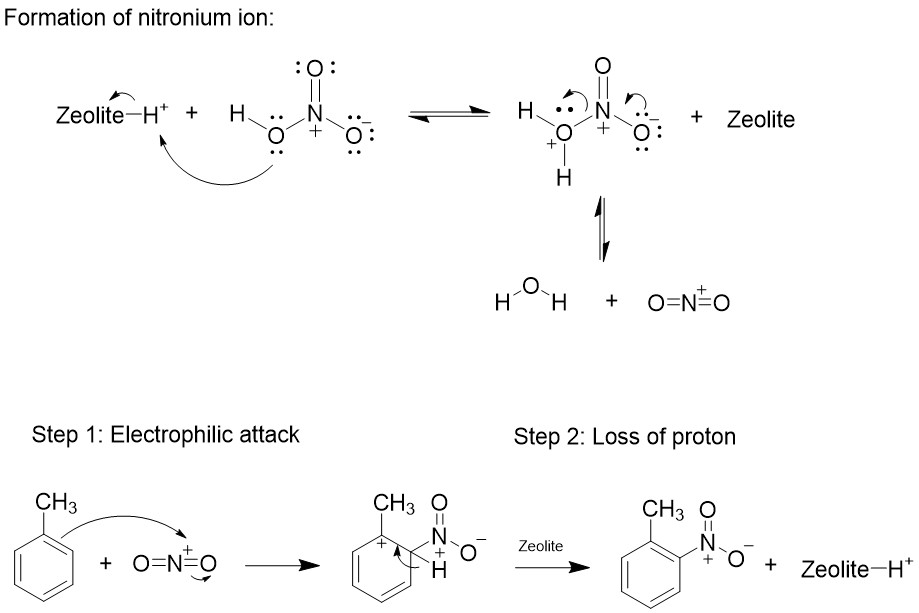
\includegraphics[width=\linewidth, scale = 0.7]{chapters/2-reaction/figures/Nitration.jpg}
    \caption{Mechanism for nitration of toluene to \ortho-nitrotoluene. Mechanism for meta and para nitrotoluene are similar, except that the nitronium ion favors the \meta and \para position of the toluene respectively.}
    \label{fig:firststep}
\end{figure}

Nitric acid interacts with the Brønsted acid sites on H-Mordenite by forming a hydrogen bond with the \ch{H+} proton [chary et al]. This results in a intermediate nitronium ion \ch{NO2+} and water molecule \ch{H2O}. The nitronium ion then undergoes electrophilic substitution with the aromatic ring of toluene to form nitrotoluenes. The electron-donating inductive effect of the methyl group on toluene favors ortho and para positions for nitrotoluene.

The nitration of toluene is governed by intrinsic kinetics under the experimental conditions [Jeeru et al]. The electrophilic substitution between the \ch{NO2+} nitronium ion and toluene is the rate determining step [carey and sundberg]. The rate equation can be defined as  

\begin{equation}
-\frac{\dd C_{Toluene}}{\dd t} = k_{2} [C_{Toluene}] [C_{Nitric Acid}] \approx k_{1} [C_{Toluene}]
\end{equation}

where $k_2$, $k_1$ are the second-order and pseudo-first order rate constant respectively. A pseudo-first order rate constant can be assumed since nitric acid is in excess. The rate constant varies with temperature according to the Arrhenius equation and this information was extracted from the Arrhenius plot in [jeeru et al]. The summary table of the activation energies and pre-exponential factors for the formation of all 3 isomers of nitrotoluene can be found in Appendix [ref]. The catalyst loading of 30 \% w/v of H-mordenite that gave the highest rate of reaction was selected from [jeeru et al].



\subsection{Hydrogenation of o-nitrotoluene}
After the production of the 3 nitrotoluene isomers, (mention separation?) ONT is mixed with propanol and hydrogenated to o-TOL in a co-current trickle bed reactor operating at 333K and 3 atm. 

\begin{scheme}[h]
    \centering
    \ch{ ONT + 3 H2 -> O{-}TOL + 2 H2O }
    \caption{ONT hydrogenation to O-TOL}
    \label{eqn: ONT hydrogenation}
\end{scheme}

include ChemDraw here
The rate equation for this equation can be defined as: 
\begin{equation}
    r = k P_{H_2}^{0.3} 
    \label{ONT rate equation}
\end{equation}
 \begin{equation}
     k = 211.69 exp(-\frac{45.52 \cdot 10^{3}}{RT} \frac{mol}{kPa^{0.3}g_{cat}s})
 \end{equation}
 
\subsection{Oxidation of p-nitrotoluene}
% Andreas

\begin{scheme}
    
\end{scheme}

\subsection{Hydrogenation of nitrobenzaldehyde and nitrobenzoic acid}

5\%w/w Pt/C catalyst in methanol, with formic acid as the reducing agent was selected.Room conditions 5\% Pt/C